\documentclass{article}
\usepackage[T1]{fontenc}
\usepackage{lmodern}
\usepackage{graphicx}
\usepackage{amsmath,amssymb}
\usepackage[a4paper,margin=2cm]{geometry}
\usepackage[absolute,overlay]{textpos}
\setlength{\TPHorizModule}{1mm}
\setlength{\TPVertModule}{1mm}
\usepackage[indonesian]{babel}
\usepackage{hyperref}
\setlength{\emergencystretch}{2em}
\title{15-Algoritma-Diffie-Hellman-2026}
\author{pdf\_ppt\_to\_latex}
\date{}

\begin{document}

% --- unit llm 1 ---
% === Halaman 1 (llm) ===

\begin{center}
Bahan kuliah IF4020 Kriptografi

{\huge \textcolor{red}{Algoritma Pertukaran Kunci Diffie-Hellman}}

\vspace{20mm}

Oleh: Rinaldi M

\vspace{10mm}

Program Studi Teknik Informatika\\
Sekolah Teknik Elektro dan Informatika\\
Institut Teknologi Bandung\\
2026
\end{center}

\newpage

% --- unit llm 2 ---
% === Halaman 2 (llm) ===

\section*{Persoalan}

\begin{itemize}
    \item Misalkan Alice dan Bob sepakat menggunakan algoritma kriptografi kunci-simetri (misalnya AES) untuk enkripsi dan dekripsi pesan.
    \item Masalahnya, Alice dan Bob harus memiliki kunci AES yang sama untuk enkripsi dan dekripsi pesan.
    \item Bagaimana cara Alice dan Bob dapat berbagi kunci AES yang sama dengan aman tanpa diketahui pihak ketiga?
    \item Solusinya: 
    \begin{enumerate}
        \item Gunakan \textit{hybrid cryptography}, atau
        \item Gunakan algoritma pertukaran kunci Diffie-Hellman
    \end{enumerate}
\end{itemize}

\newpage

% --- unit llm 3 ---
% === Halaman 3 (llm) ===

\section*{Hybrid Cryptography}

\begin{itemize}
    \item Alice dan Bob sepakat mengenkripsi dan mendekripsi pesan dengan algoritma kriptografi simetri (misalkan AES).
    \item Bagaimana cara Bob dapat mengetahui kunci AES yang digunakan oleh Alice (kunci AES)?
    \item Solusinya adalah dengan menggunakan \textit{hybrid cryptography}.
    \item \textit{Hybrid cryptography}: menggabungkan kriptografi kunci-simetri (misalkan AES) dengan kriptografi kunci-publik (misalkan RSA).
    \item Caranya sebagai berikut:
    \begin{enumerate}
        \item Alice memiliki sepasang kunci privat ($\text{SK}_{\text{Alice}}$) dan kunci publik ($\text{PK}_{\text{Alice}}$) miliknya.
        \item Bob juga memiliki sepasang kunci privat ($\text{SK}_{\text{Bob}}$) dan kunci publik ($\text{PK}_{\text{Bob}}$) miliknya.
    \end{enumerate}
\end{itemize}

\newpage

% --- unit llm 4 ---
% === Halaman 4 (llm) ===

\begin{enumerate}
  \item[3)] Alice membangkitkan kunci rahasia (K) untuk enkripsi pesan dengan AES
  \item[4)] Alice mengenkripsi K dengan RSA menggunakan kunci publik Bob (PK$_{Bob}$).
  \[ E\_RSA_{PKbob}(K) = CK \]
  \item[5)] Alice mengenkripsi pesan M dengan AES menggunakan K,
  \[ E\_AES_{K}(M) = CM \]
  lalu mengirim CK dan CM kepada Bob.
  \item[6)] Bob mendekripsi CK dengan RSA menggunakan kunci privatnya (SK$_{Bob}$)
  \[ D\_RSA_{SKbob}(CK) = K \]
  \item[7)] Selanjutnya Bob mendekripsi pesan CM dengan AES menggunakan K
  \[ D\_AES_{K}(CM) = M \]
\end{enumerate}

\vspace{10mm}
\centering{Rinaldi M/II4020 Kriptografi}

\newpage

% --- unit llm 5 ---
% === Halaman 5 (llm) ===

\begin{center}
\Huge Hybrid Cryptography
\end{center}

\vspace{80mm}

Sumber: \url{https://www.mayurpahwa.com/2018/12/hybrid-cryptography.html}

\vspace{5mm}

\begin{center}
Rinaldi M/I14020 Kriptografi
\end{center}

% deskripsi: Diagram alur kriptografi hibrida yang menunjukkan proses pengiriman pesan dari Alice ke Bob, melibatkan enkripsi dengan kunci rahasia K, enkripsi kunci K dengan kunci publik Bob (PK_Bob), dan dekripsi kembali menggunakan kunci privat Bob (SK_Bob).
% bbox normalisasi: [0.1700, 0.1800, 0.8800, 0.7500]
\begin{textblock*}{149.10mm}(35.70mm,53.46mm)
\noindent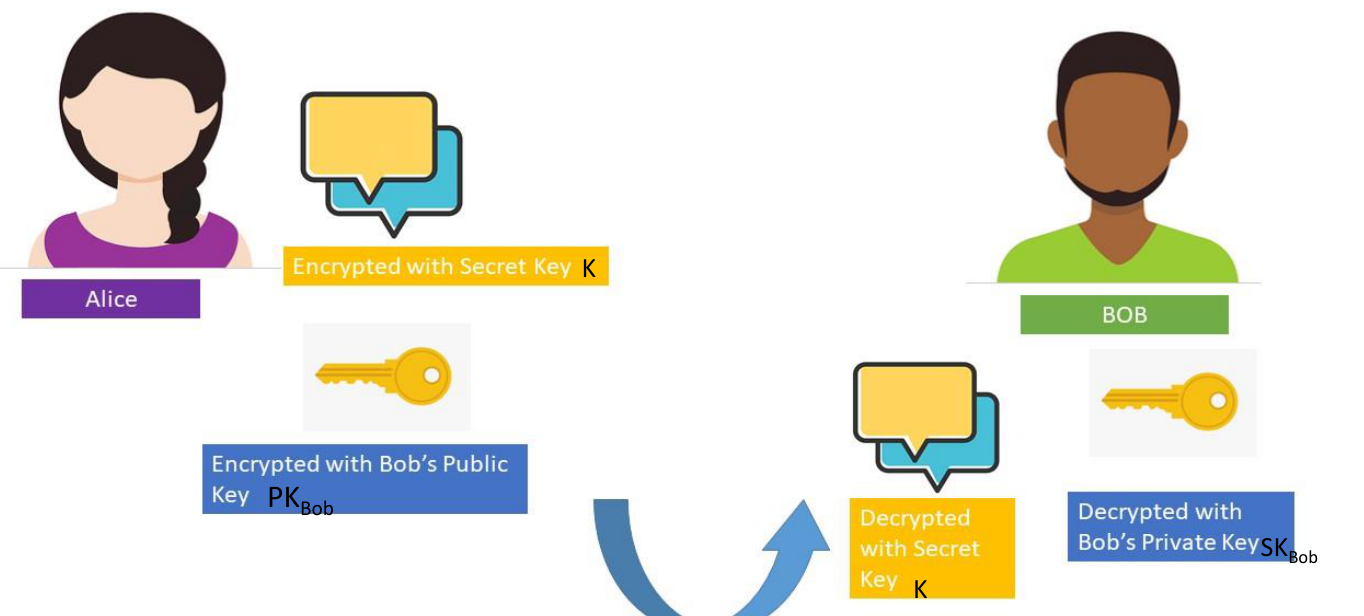
\includegraphics[width=149.10mm,height=169.29mm]{images/llm/page_005_img_01.png}%
\end{textblock*}

\newpage

% --- unit llm 6 ---
% === Halaman 6 (llm) ===

\begin{center}
\Huge Hybrid Cryptography
\end{center}

\vspace{100mm}

\noindent \url{https://www.researchgate.net/figure/Illustration-of-a-hybrid-cryptosystem_fig8_327799148}

\vspace{5mm}

\noindent Rinaldi M/II4020 Kriptografi

% deskripsi: Diagram alur kriptografi hibrida yang menunjukkan proses enkripsi oleh Bob menggunakan AES dan RSA, serta proses dekripsi oleh Alice.
% bbox normalisasi: [0.1800, 0.1100, 0.7400, 0.8500]
\begin{textblock*}{117.60mm}(37.80mm,32.67mm)
\noindent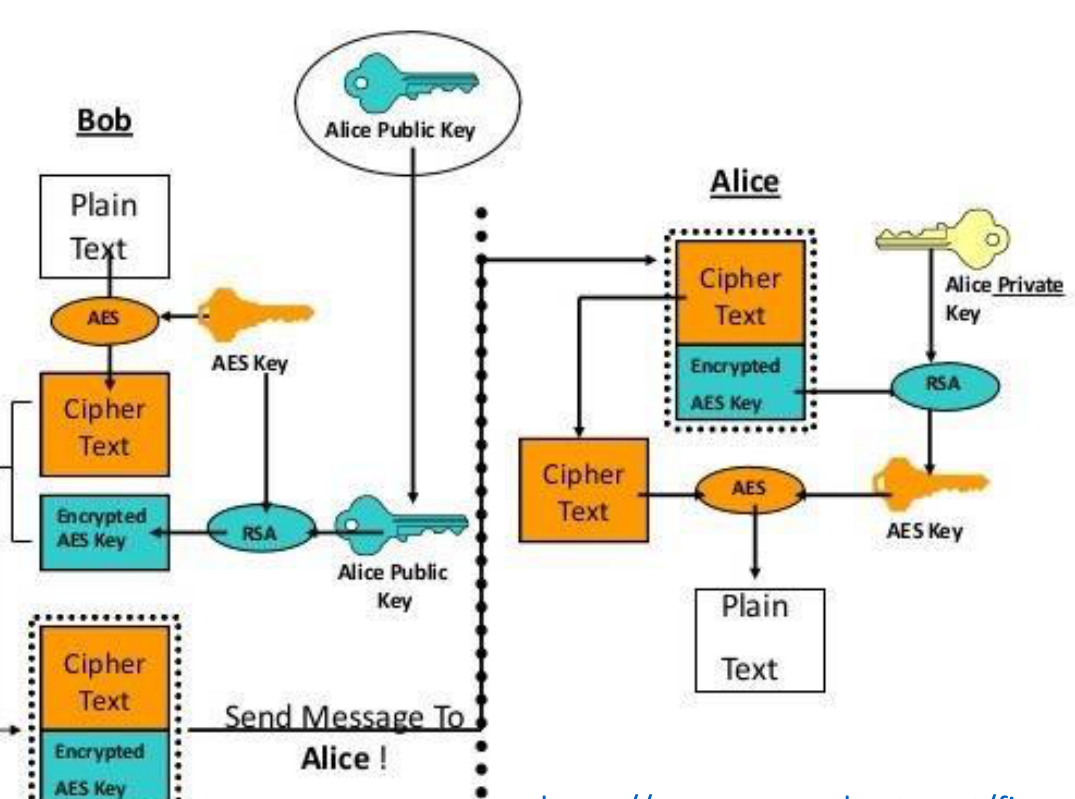
\includegraphics[width=117.60mm,height=219.78mm]{images/llm/page_006_img_01.png}%
\end{textblock*}

\newpage

% --- unit llm 7 ---
% === Halaman 7 (llm) ===

\begin{itemize}
  \item Alternatif selain \textit{hybrid cryptography} adalah menggunakan algoritma pertukaran kunci Diffie-Hellman.
\end{itemize}

\newpage

% --- unit llm 8 ---
% === Halaman 8 (llm) ===

\section*{Algoritma Pertukaran Kunci Diffie-Hellman}

\vspace{145.83mm}

\begin{itemize}
    \item Algoritma (lebih tepat disebut \textbf{protokol}) \textbf{pertukaran kunci Diffie-Hellman} (DH) berguna untuk berbagi kunci rahasia yang sama antara dua entitas yang berkomunikasi.
    \vspace{40mm}
    \item Kunci rahasia selanjutnya digunakan untuk mengenkripsi pesan-pesan dengan algoritma kriptografi kunci-simetri (misalnya DES, AES, dll).
    \item Keamanan algoritma DH didasarkan pada sulit menghitung logaritma diskrit dari sebuah bilangan bulat besar.
\end{itemize}

\begin{center}
    Rinaldi M/II4020 Kriptografi
\end{center}

% deskripsi: Diagram ilustrasi proses pertukaran kunci Diffie-Hellman antara Bob dan Alice dengan adanya Eve sebagai penyadap, menunjukkan aliran nilai Val1, Val2, dan hasil akhir berupa same shared (secret)-key.
% bbox normalisasi: [0.5700, 0.3360, 0.9820, 0.8270]
\begin{textblock*}{86.52mm}(119.70mm,99.79mm)
\noindent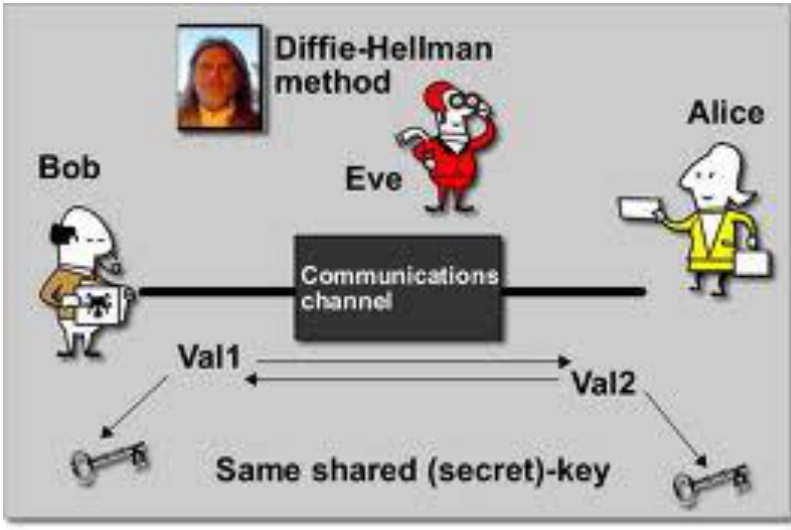
\includegraphics[width=86.52mm,height=145.83mm]{images/llm/page_008_img_01.png}%
\end{textblock*}

\newpage

% --- unit llm 9 ---
% === Halaman 9 (llm) ===

\begin{itemize}
    \item Algoritma pertukaran kunci Diffie-Hellman dipublikasikan oleh Whitfield Diffie dan Martin Hellman pada tahun 1976
\end{itemize}

\vspace{50mm}

Whitfield \textbf{Diffie} dan Martin \textbf{Hellman}

\vspace{10mm}
Rinaldi M/II4020 Kriptografi

% deskripsi: Foto potret Whitfield Diffie dan Martin Hellman berdampingan
% bbox normalisasi: [0.2400, 0.3100, 0.6920, 0.8110]
\begin{textblock*}{94.92mm}(50.40mm,92.07mm)
\noindent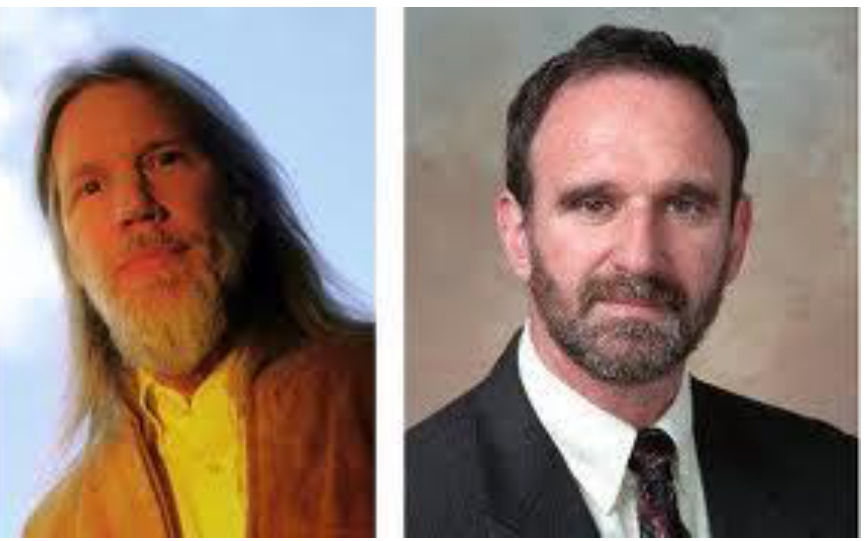
\includegraphics[width=94.92mm,height=148.80mm]{images/llm/page_009_img_01.png}%
\end{textblock*}

\newpage

% --- unit llm 10 ---
% === Halaman 10 (llm) ===

\begin{itemize}
    \item Analogi pertukaran kunci Diffie-Hellman adalah seperti pertukaran cat antara dua orang (Alice dan Bob).
    \item Mula-mula Alice dan Bob menyepakati cat bersama yang warnanya tidak perlu rahasia (misalnya cat berwarna kuning)
    \item Masing-masing Alice dan Bob memiliki warna lain yang rahasia (dalam hal ini merah dan biru \textit{cyan})
    \item Alice dan Bob mencampurkan cat kuning dengan cat rahasia mereka masing-masing. Misalkan hasil pencampurannya adalah cat oranye dan cat biru terang
    \item Kemudian Alice dan Bob saling mempertukarkan cat hasil pencampuran tersebut (dikirim melalui transportasi umum).
    \item Selanjutnya, Alice dan Bob mencampurkan lagi cat rahasianya masing-masing dengan cat hasil pertukaran tersebut.
    \item Sekarang Alice dan Bob memiliki cat berwarna sama yang rahasia.
\end{itemize}

\vspace{10mm}

\begin{center}
    Rinaldi M/IL4020 Kriptografi
\end{center}

% deskripsi: Diagram ilustrasi analogi pertukaran kunci Diffie-Hellman menggunakan pencampuran warna cat antara Alice dan Bob.
% bbox normalisasi: [0.6300, 0.3600, 0.9800, 0.9300]
\begin{textblock*}{73.50mm}(132.30mm,106.92mm)
\noindent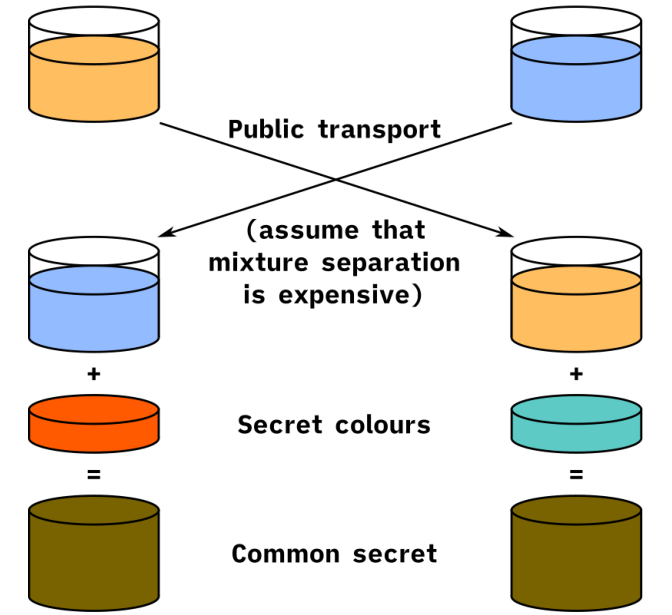
\includegraphics[width=73.50mm,height=169.29mm]{images/llm/page_010_img_01.png}%
\end{textblock*}

\newpage

% --- unit llm 11 ---
% === Halaman 11 (llm) ===

\section*{Parameter umum Diffie-Hellman}

\begin{itemize}
    \item Misalkan dua entitas yang berkomunikasi adalah Alice dan Bob.
    \item Mula-mula Alice dan Bob menyepakati sebuah bilangan prima $p$, dan sebuah bilangan bulat $g$, sedemikian sehingga $g < p$ dan $g$ adalah akar primitif dari $p$.
    \item Nilai $p$ dan $g$ tidak perlu rahasia. Bahkan, Alice dan Bob dapat membicarakannya melalui saluran publik yang tidak aman sekalipun.
\end{itemize}

\vspace{10mm}

\begin{center}
Rinaldi M/II4020 Kriptografi
\end{center}

\newpage

% --- unit llm 12 ---
% === Halaman 12 (llm) ===

\section*{Algoritma Pertukaran Kunci Diffie-Hellman}

\begin{enumerate}
  \item Alice membangkitkan bilangan bulat acak $a$ dan mengirim hasil perhitungan berikut kepada Bob:
  \[ A = g^a \bmod p \quad (a = \text{kunci privat Alice, } A = \text{kunci publik Alice}) \]
  \item Bob membangkitkan bilangan bulat acak $b$ dan mengirim hasil perhitungan berikut kepada Alice:
  \[ B = g^b \bmod p \quad (b = \text{kunci privat Bob, } B = \text{kunci publik Bob}) \]
  \item Alice menghitung
  \[ K = B^a \bmod p \quad (K = g^{ab} \bmod p) \]
  \item Bob menghitung
  \[ K = A^b \bmod p \quad (K = g^{ab} \bmod p) \]
\end{enumerate}

\begin{itemize}
  \item Jika perhitungan dilakukan dengan benar, maka $K = g^{ab} \bmod p$. Alice dan Bob sekarang memiliki kunci rahasia yang sama, yaitu $K$.
\end{itemize}

\newpage

% --- unit llm 13 ---
% === Halaman 13 (llm) ===

Alice \vspace{5mm} Bob \vspace{5mm} Rinaldi M/II4020 Kriptografi

\vspace{117.02mm}

% deskripsi: Diagram pertukaran kunci Diffie-Hellman yang menunjukkan langkah-langkah perhitungan Alice dan Bob menggunakan parameter publik g dan p untuk menghasilkan kunci rahasia bersama K.
% bbox normalisasi: [0.1610, 0.5300, 0.8380, 0.9240]
\begin{textblock*}{142.17mm}(33.81mm,157.41mm)
\noindent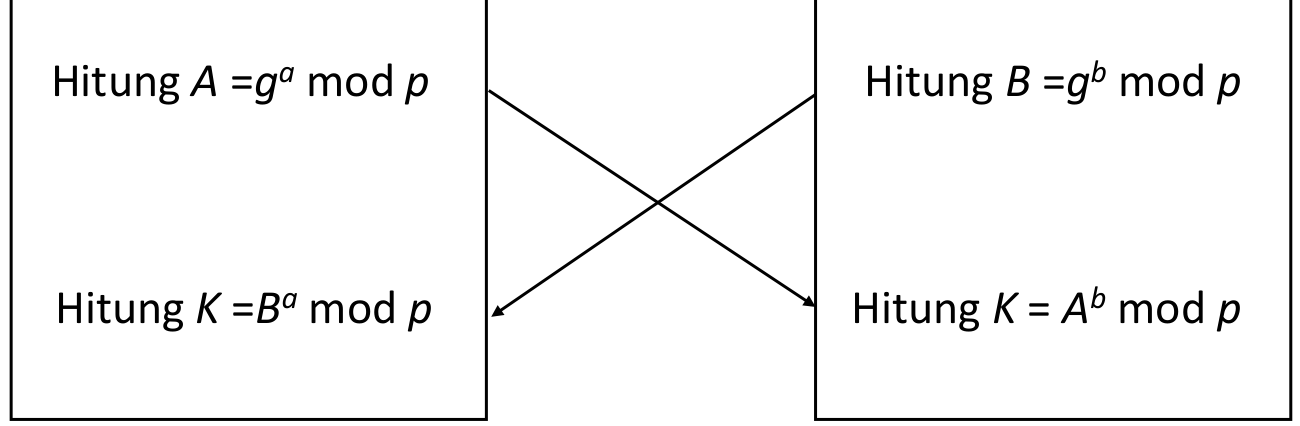
\includegraphics[width=142.17mm,height=117.02mm]{images/llm/page_013_img_01.png}%
\end{textblock*}

\newpage

% --- unit llm 14 ---
% === Halaman 14 (llm) ===

\begin{itemize}
  \item Eve (seorang kriptanalis) yang menyadap pembicaraan Alice dan Bob tidak dapat menghitung $K$.
  \item Sebab Eve hanya memiliki informasi $p, g, A$ dan $B$ yang semuanya tidak rahasia, tetapi ia tidak mengetahui nilai $a$ atau $b$.
  \item Untuk mengetahui $a$, Eve perlu melakukan perhitungan untuk menemukan $a$ dari persamaan $A = g^a \pmod{p}$. ($a$ adalah logaritma diskrit dari $A$ dalam modulus $p$)
  \item Sekali $a$ diketahui, maka selanjutnya Eve menggunakannya untuk menghitung kunci rahasia $K = B^a \pmod{p}$.
  \item Kabar baiknya, logaritma diskrit bilangan bulat yang besar sangat sulit dihitung. Jadi, Eve tidak dapat menemukan kunci $K$.
\end{itemize}

\vfill
\centering Rinaldi M/II4020 Kriptografi

\newpage

% --- unit llm 15 ---
% === Halaman 15 (llm) ===

Contoh: Alice dan Bob menyepakati $p = 353$ dan $g = 3$ ( $3 < 353$, dan $3$ adalah akar primitif $353$)

\begin{enumerate}
    \item Alice memilih $a = 97$ dan menghitung
    \[ A = g^a \pmod p = 3^{97} \pmod{353} = 40 \]
    Alice mengirim $A$ kepada Bob.
    \item Bob memilih $b = 233$ dan menghitung
    \[ B = g^b \pmod p = 3^{233} \pmod{353} = 248 \]
    Bob mengirim $B$ kepada Alice.
    \item Alice menghitung kunci rahasia $K$,
    \[ K = B^a \pmod p = 248^{97} \pmod{353} = 160 \]
    \item Bob menghitung kunci rahasia $K$,
    \[ K = A^b \pmod p = 40^{233} \pmod{353} = 160 \]
\end{enumerate}

\vspace{30mm}

Jadi, Alice dan Bob sekarang sudah mempunyai kunci rahasia yang sama, yaitu $K = 160$. Mereka dapat menggunakan $K$ sebagai kunci enkripsi dan dekripsi pesan dengan algoritma kunci simetri.

\begin{center}
    Rinaldi M/II4020 Kriptografi
\end{center}

% deskripsi: Diagram alur pertukaran kunci Diffie-Hellman antara Alice dan Bob, menunjukkan pengiriman parameter g, p dan nilai A, B untuk menghitung kunci rahasia K.
% bbox normalisasi: [0.5200, 0.3400, 0.9700, 0.7300]
\begin{textblock*}{94.50mm}(109.20mm,100.98mm)
\noindent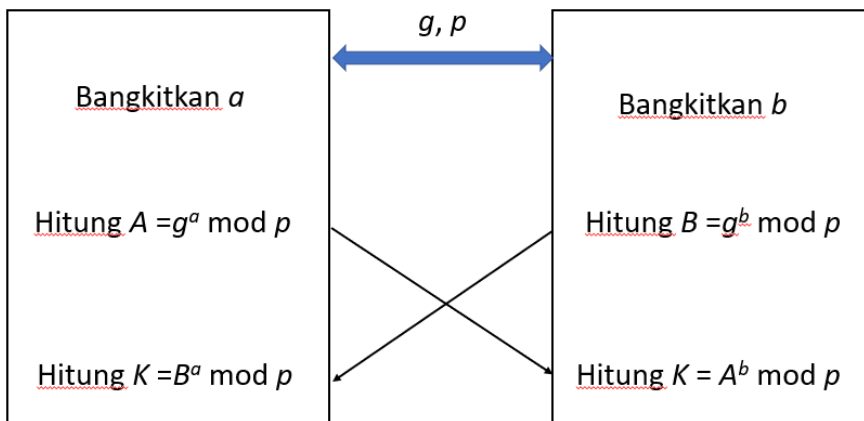
\includegraphics[width=94.50mm,height=115.83mm]{images/llm/page_015_img_01.png}%
\end{textblock*}

\newpage

% --- unit llm 16 ---
% === Halaman 16 (llm) ===

\vspace{213.84mm}

\begin{itemize}
    \item Contoh lain:
\end{itemize}

\vspace{10mm}

\vspace{60mm}

Sumber: http://sspai.com/26497 \hfill Rinaldi M/II4020 Kriptografi

% deskripsi: Diagram proses pertukaran kunci Diffie Hellman antara Alice dan Bob dengan keberadaan penyadap Evil Eve, menunjukkan langkah-langkah perhitungan matematika dari pembuatan nomor acak hingga penentuan Secret Key.
% bbox normalisasi: [0.1400, 0.1200, 0.8300, 0.8400]
\begin{textblock*}{144.90mm}(29.40mm,35.64mm)
\noindent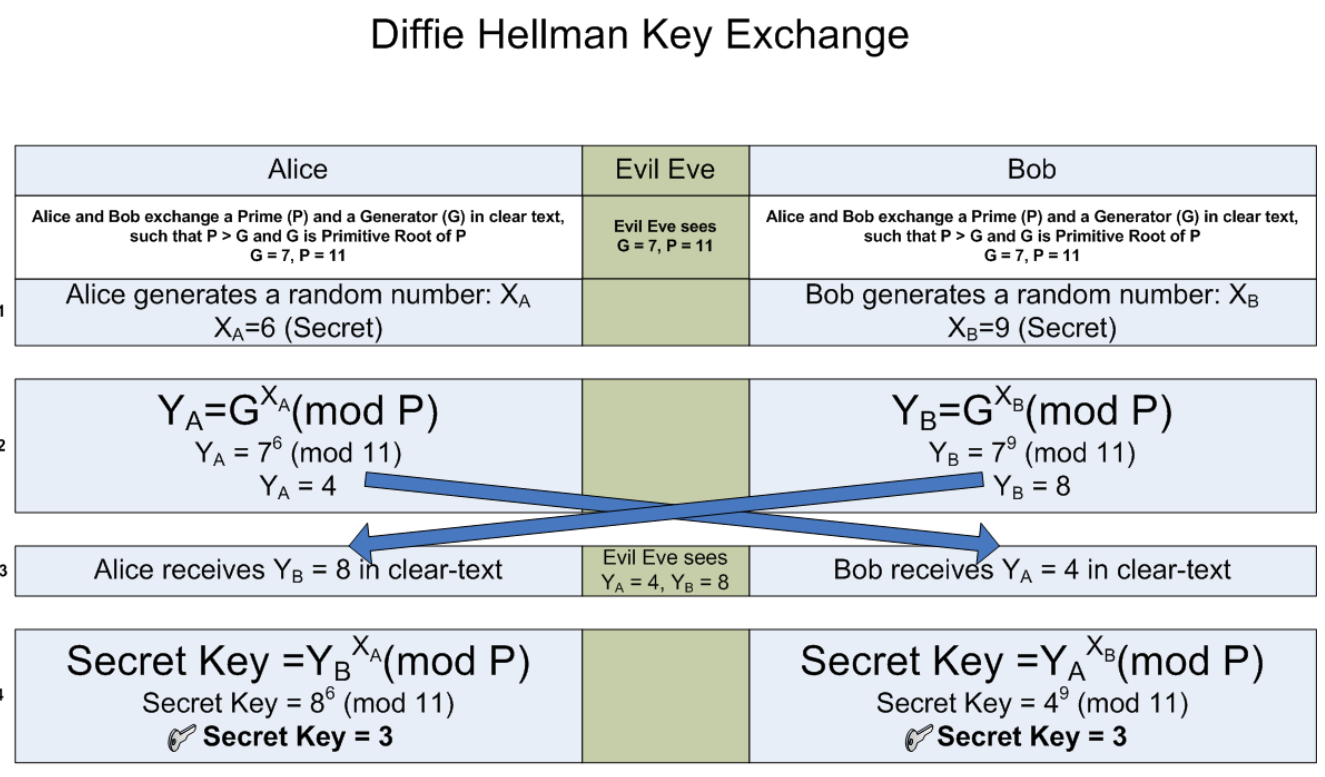
\includegraphics[width=144.90mm,height=213.84mm]{images/llm/page_016_img_01.png}%
\end{textblock*}

\newpage

% --- unit llm 17 ---
% === Halaman 17 (llm) ===

\section*{Serangan pada Diffie-Hellman}

\begin{itemize}
    \item Pertukaran kunci Diffie-Hellman hanya aman terhadap serangan pasif, misalnya penyadapan (\textit{eavesdropping}).
    \item Eva yang menyadap komunikasi antara Alice dan Bob hanya mengetahui nilai $g, p, A$ dan $B$ (semuanya publik). Dia tidak dapat mendeduksi $a$ dan $b$ (kunci privat Alice dan Bob) dari nilai-nilai publik tersebut. Untuk mendeduksi $a$ dan $b$, Eva harus dapat menghitung logaritma diskrit dari persamaan
    \[ A = g^a \pmod{p} \text{ atau } B = g^b \pmod{p} \]
    \item Namun, Diffie-Hellman tidak tahan terhadap serangan aktif seperti \textit{man-in-the-middle attack}.
    \item Misalkan Mallory mengintervensi komunikasi antara Alice dan Bob. Kepada Alice Malllory menyamar (\textit{impersonation}) sebagai Bob, dan kepada Bob Mallory menyamar sebagai Alice.
\end{itemize}

\vfill
\begin{center}
    Rinaldi M/II4020 Kriptografi
\end{center}

\newpage

% --- unit llm 18 ---
% === Halaman 18 (llm) ===

\begin{itemize}
    \item Gambar \textit{man-in-the-middle attack} berikut memperlihatkan cara Mallory menyepakati kunci yang sama dengan Alice ($K_1 = g^{am} \pmod{p}$) dan menyepakati kunci yang sama dengan Bob ($K_2 = g^{bm} \pmod{p}$)
    \vspace{40mm}
    \item Ketika Alice mengirim $g^a \pmod{p}$ kepada Bob, Mallory mengintersepsi komunikasi dan menggantikannya dengan $g^m \pmod{p}$ lalu mengirimkannya kepada Bob
    \item Ketika Bob mengirim $g^b \pmod{p}$ kepada Alice, Mallory mengintersepsi komunikasi dan menggantikannya dengan $g^m \pmod{p}$ lalu mengirimkannya kepada Alice.
    \item Alice menghitung $K_1 = g^{am} \pmod{p}$, sama dengan yang dihitung Mallory, $K_1 = g^{am} \pmod{p}$
    \item Bob menghitung $K_2 = g^{bm} \pmod{p}$, sama dengan yang dihitung Mallory, $K_2 = g^{bm} \pmod{p}$
    \item Selanjutnya Mallory mengetahui pesan2 rahasia dari Alice dan dari Bob yang dienkripsi dengan dengan kunci $K_1$ dan $K_2$ tersebut
\end{itemize}

\vspace{10mm}

Sumber gambar: \url{https://textbook.cs161.org/crypto/key-exchange.html}

\hfill Rinaldi M/I4020 Kriptografi

% deskripsi: Diagram serangan man-in-the-middle pada pertukaran kunci Diffie-Hellman yang melibatkan Alice, Mallory, dan Bob.
% bbox normalisasi: [0.5200, 0.2700, 0.9500, 0.8300]
\begin{textblock*}{90.30mm}(109.20mm,80.19mm)
\noindent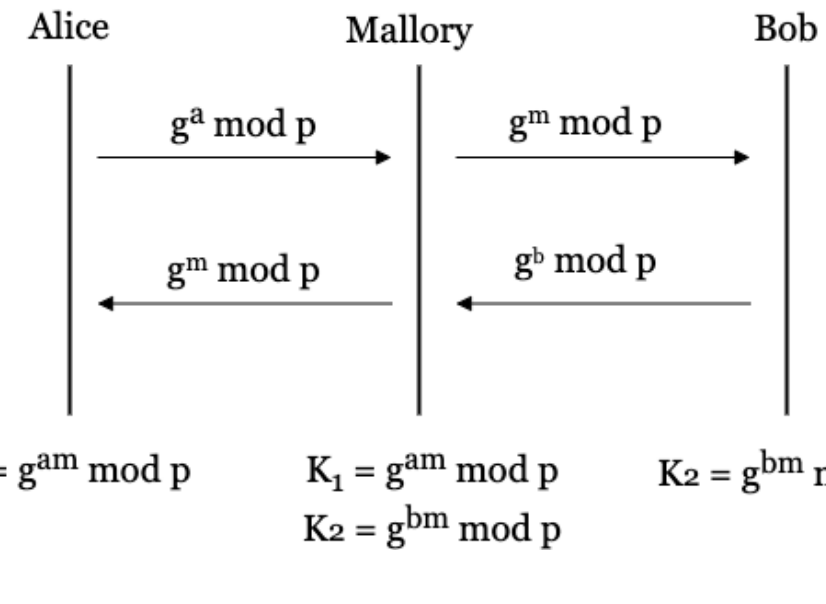
\includegraphics[width=90.30mm,height=166.32mm]{images/llm/page_018_img_01.png}%
\end{textblock*}

\newpage

% --- unit llm 19 ---
% === Halaman 19 (llm) ===

\section*{Pertukaran kunci Diffie-Hellman untuk tiga pihak (Alice, Bob, dan Carol)}

\begin{enumerate}
  \item Alice, Bob, dan Carol menyepakati $p$ dan $g$.
  \item Alice, Bob, dan Carol membangkitkan kunci privat masing-masing, $a$, $b$, dan $c$.
  \item Alice menghitung $g^a \pmod p$ dan mengirimkannya kepada Bob.
  \item Bob menghitung $(g^a)^b \pmod p = g^{ab} \pmod p$ dan mengirimkannya kepada Carol.
  \item Carol menghitung $K = (g^{ab})^c \pmod p = g^{abc} \pmod p$.
  \item Bob menghitung $g^b \pmod p$ dan mengirimkannya kepada Carol.
  \item Carol menghitung $(g^b)^c \pmod p = g^{bc} \pmod p$ dan mengirimkannya kepada Alice.
  \item Alice menghitung $K = (g^{bc})^a \pmod p = g^{bca} \pmod p = g^{abc} \pmod p$.
  \item Carol menghitung $g^c \pmod p$ dan mengirimkannya kepada Alice.
  \item Alice menghitung $(g^c)^a \pmod p = g^{ca} \pmod p$ dan mengirimkannya kepada Bob.
  \item Bob menghitung $K = (g^{ca})^b \pmod p = g^{cab} \pmod p = g^{abc} \pmod p$.
  \item Sekarang Alice, Bob, dan Carol sudah memiliki kunci rahasia yang sama, yaitu $K$
\end{enumerate}

\newpage

% --- unit llm 20 ---
% === Halaman 20 (llm) ===

\begin{itemize}
    \item Algoritma Diffie-Hellman dipakai di dalam protokol SSL dan TLS. SSL/TLS digunakan untuk mengamankan komunikasi di internet antara \textit{client} dan \textit{server}.
    \item Pada tahun 2002, Hellman menyarankan algoritma DH diberi nama algoritma pertukaran kunci \textbf{Diffie--Hellman--Merkle} sebagai penghargaan terhadap kontribusi Ralph Merkle dalam penemuan kriptografi kunci-publik:
    \item Hellman menulis:
    \begin{quote}
    \textit{The system...has since become known as Diffie--Hellman key exchange. While that system was first described in a paper by Diffie and me, it is a public key distribution system, a concept developed by Merkle, and hence should be called 'Diffie--Hellman--Merkle key exchange' if names are to be associated with it. I hope this small pulpit might help in that endeavor to recognize Merkle's equal contribution to the invention of public key cryptography.[7]}
    \end{quote}
\end{itemize}

\begin{flushright}
Sumber: Wikipedia
\end{flushright}

\newpage

% --- unit llm 21 ---
% === Halaman 21 (llm) ===

\textbf{The IEEE Koji Kobayashi Computers and Communications Award}\
The 1999 award was given to Diffie, Hellman and Merkle \"For the revolutionary invention of public key cryptosystems which form the foundation for privacy, integrity and authentication in modern communication systems.\"
The 2000 award was given to Rivest, Shamir and Adleman \"For the revolutionary invention of the RSA public key cryptosystem which is the first to be widely-adopted.\"

\vspace{50mm}

From left to right: Adi Shamir, Ron Rivest, Len Adleman, Ralph Merkle, Martin Hellman, and Whit Diffie (Picture courtesy of Eli Biham, taken at the presentation on Monday August 21 at Crypto 2000, an IACR conference)

\centering{Rinaldi M/II4020 Kriptografi}\
\centering{\textcolor{red}{Sumber: http://www.merkle.com/merkleDir/KobayashiAward.html}}

% deskripsi: Foto para penerima Penghargaan IEEE Koji Kobayashi Computers and Communications, yang terdiri dari Adi Shamir, Ron Rivest, Len Adleman, Ralph Merkle, Martin Hellman, dan Whit Diffie.
% bbox normalisasi: [0.1800, 0.2600, 0.7440, 0.7760]
\begin{textblock*}{118.44mm}(37.80mm,77.22mm)
\noindent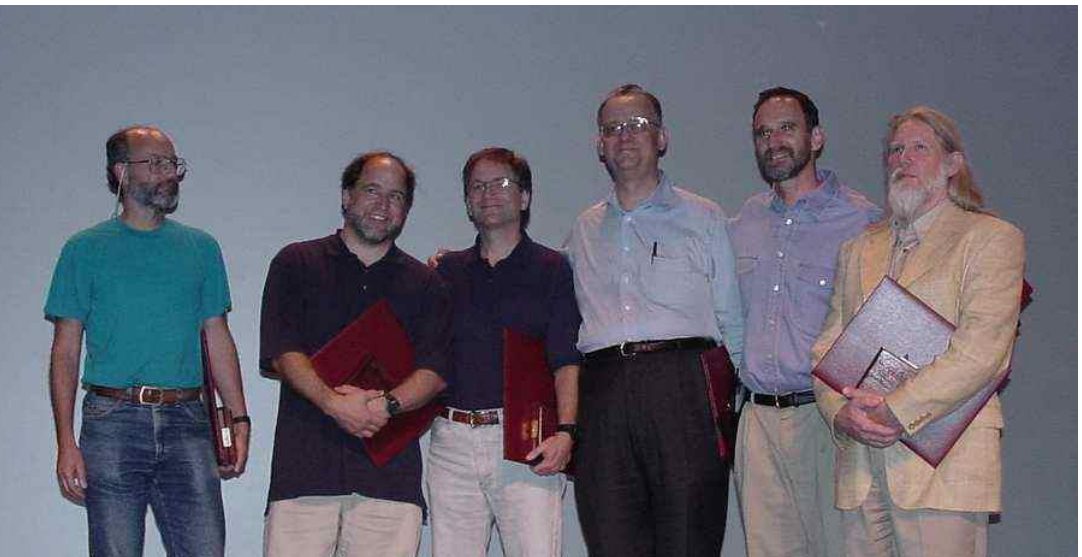
\includegraphics[width=118.44mm,height=153.25mm]{images/llm/page_021_img_01.png}%
\end{textblock*}

\newpage

% --- unit llm 22 ---
% === Halaman 22 (llm) ===

Demo DH online: https://asecuritysite.com/encryption/diffie

\section*{Diffie-Hellman Example}

\vspace{201.96mm}

[Encryption Home][Home]

Diffie-Hellman is a standard method of Alice and Bob being able to communicate, and end up with the same secret encryption key. It is used in many applications, and uses two numbers (G and N) for the first part of the calculation (of which N must be a prime number):

[Related Lecture] [Tutorial] [Software Tutorial] [Software Lecture] [Theory] [Blog] [Picking G value]

G: 1601 \\
N: 4789

\vspace{10mm}

Next Bob and Alice will generate two random numbers (X and Y), calculate an X value and a Y value, respectively:

\begin{tabular}{ll} 
Bob's X Value & 20 \\
Bob's random value & \\
Bob's A value & 2716 \\
$A = G^{x} \pmod{N}$ & \\
\end{tabular} 
\begin{tabular}{ll} 
Alice's Y value & 4 \\
Alice's random value & \\
Alice's B value & 1302 \\
$B = G^{y} \pmod{N}$ & \\
\end{tabular}

% deskripsi: Tampilan antarmuka web simulasi Diffie-Hellman yang menunjukkan input nilai G, N serta perhitungan nilai A dan B untuk Bob dan Alice.
% bbox normalisasi: [0.0400, 0.2100, 0.8500, 0.8900]
\begin{textblock*}{170.10mm}(8.40mm,62.37mm)
\noindent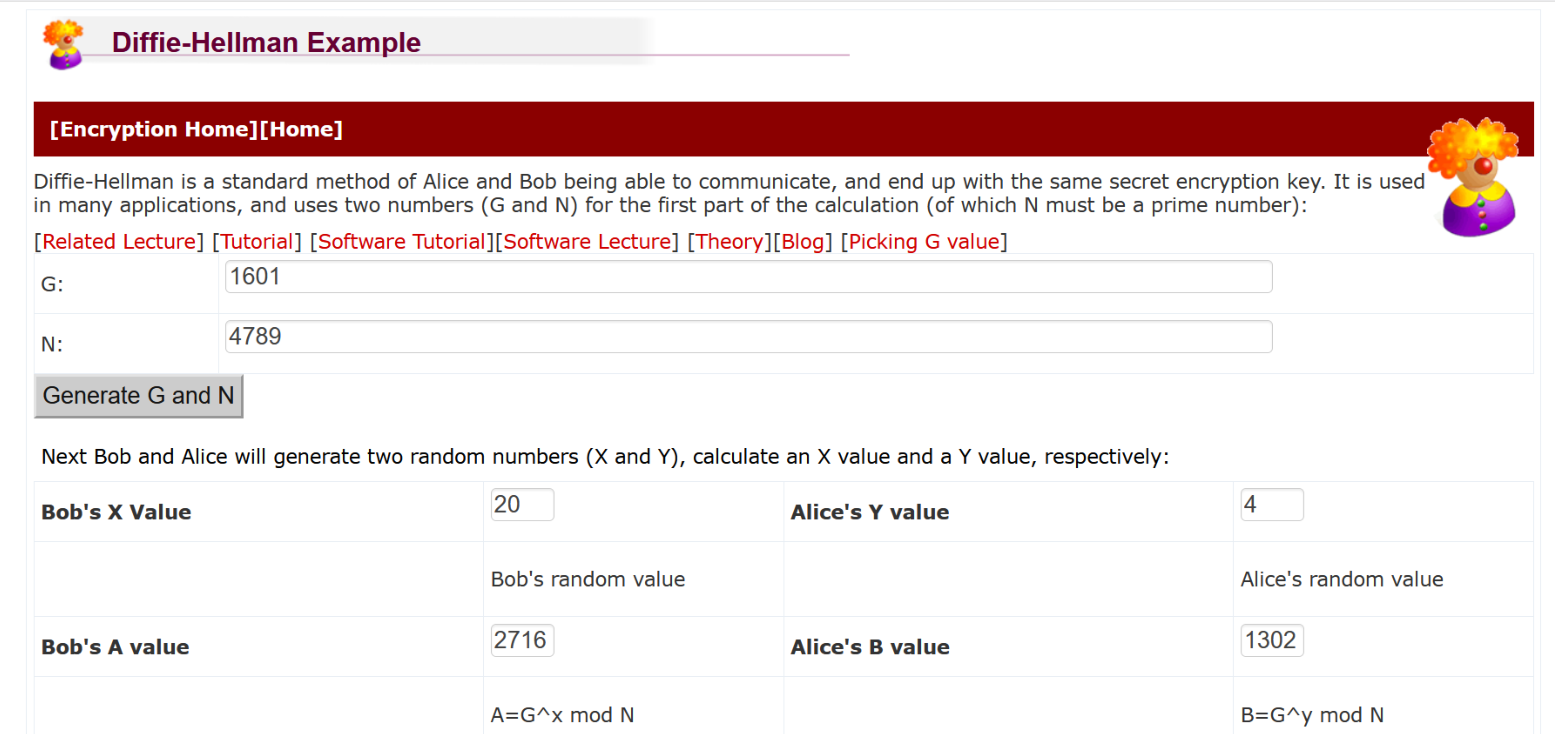
\includegraphics[width=170.10mm,height=201.96mm]{images/llm/page_022_img_01.png}%
\end{textblock*}

\end{document}
